\section{Introduction}
The last PF candidates that are reconstructed are hadrons. The calorimetric measurements, energy clusters, are the only way to identify neutral hadrons while these measurements complement the track measurements for charged hadrons. When hadrons enter calorimeters, some hadrons start showering in the ECAL and extend to the HCAL (EH-hadrons), while others do not have nuclear interactions until the HCAL (H-hadrons). Hadronic showers have electromagnetic (EM) and hadronic (HAD) components. A key feature of hadronic showers is the fluctuations in the invisible energy lost in binding energy or target recoil, particle type, and particle multiplicity generated by the same incident particle.%source
For the previous reasons, the energy response for hadrons was non-linear.    
 
This chapter introduces the details of testing an ML technique, Dynamic reduction network (DRN), in performing a PF hadron cluster calibration.    

%---------------------------------------
%1source https://www.desy.de/~schleper/lehre/Det_Dat/SS_2018/06_lecture_calorimetry_HAD.pdf

\section{Graph Neural Network} %source
Graph neural network (GNN) is a type of NN used to process data that can be represented as graphs. Compared to other kinds of NN, GNN can be applied to sparse data, such as rechits.%(introduce rechits)
As shown in (fig), a graph consists of nodes and edges. Nodes represent the objects, and edges reflect the relationship between the nodes. In our case, rechits are the nodes, and the edges represent their connection in a cluster. Graph convolutional networks (GCNs)(source) relies on message-passing methods to exchange information and messages between the neighbors (rechits). GCNs work through two steps: First, each node creates a feature vector representing the message it wants to share with others. In the second step, messages are sent to the neighbors so that each node learns about its neighbors and itself. In (fig), there is a visualization of message passing.     

\section{Datasets Description}
The second part of this thesis focuses on correcting charged hadrons PF clusters for Run3. Single Pion gun Monte Carlo (MC) samples are used for this calibration. The datasets are centrally produced and reconstructed under CMSSW 12.6.4 (126X) under 23 conditions. These samples are also available through the DAS web page and cover energy ranges of 2-200 GeV and 200-500 GeV. For training the ML model, the data are divided to EH-hadrons and H-hadrons. (add figure shows EH.H location in CMS) 

\section{PF Cluster Regression Using DRN}
Dynamic Reduction Network (DRN) (source) is based on the Graph neural network (GNN) used in this thesis to reconstruct hadron (Pion) showers in the calorimeters. A schematic of the DRN is shown in (fig), and a summary of the information flow from the inputs to the targets is as follows:   

First, The input features, the coordinates (x, y, and z) and energy (E) of rechits in a point cloud image of the detectors are mapped onto a 64-dimensional latent space using a fully connected neural network (FCNN).  The FCNN is a multi-layer perceptron (MLP) encoder with a depth of three layers connected by activation functions (exponential linear unit, ELU).

Second, High-level features are learned using the GNN techniques by repeating the following steps twice: starting with a graph generation (KNN) step: Each point in the point cloud in the 64-dimensional latent space is connected to its 16 nearest neighboring nodes, including itself, to form graphs. We have 3D point clouds, scattered collections of points (clusters) (source.)Each node (input) is connected to its K nearest neighbors in the feature space. The direct graph has vertices and edges.%(k=100)
Then, graph convolution step: The resulting graphs are processed using the operation “EdgeConv,” where two-layer (here 2 or 3) fully connected networks are used to create messages sent along the edges of the graph. These messages are aggregated at each node in the graph to form the new node feature.%(define edge features)
Next, graph clustering and pooling: Graph clustering uses the Graclus clustering algorithm and pooling step. In this step, the updated features are weighted by distance, and the clusters are combined using a max-pooling strategy to form a single point.  

The final set of nodes is reduced using global max-pooling and passed through an FCNN to obtain the final target, which in our case is the pion energy.   
\section{Results}
we present the results of response and resolution (from DRN vs Chi2) in  both Barrel region and endcap region.

\subsection{EH Hadrons}
The presented results are for the training target ratioflip

\usepackage{lscape}
\begin{landscape}  
\begin{figure}
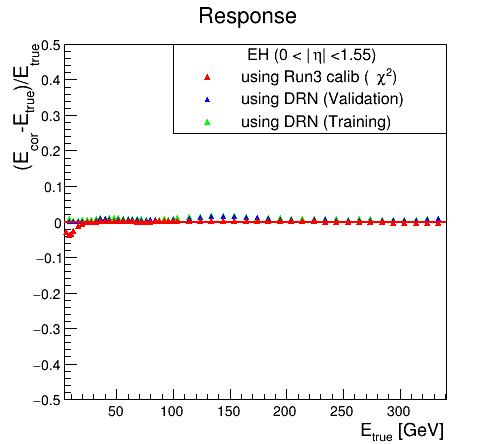
\includegraphics[width=0.495\textwidth]{./plots_pdf/HCAL_plots/Trained_target_ratioflip_0_500_10/pdf/EH_barrel/barrel_corrEtaBarrelEcalHcal.png}
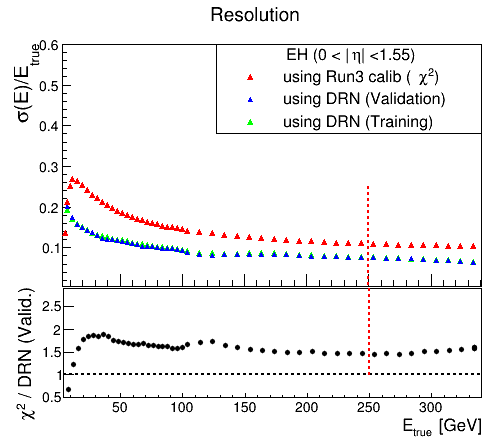
\includegraphics[width=0.495\textwidth]{./plots_pdf/HCAL_plots/Trained_target_ratioflip_0_500_10/pdf/EH_barrel/barrel_corrEtaBarrelEcalHcal_reso.png}
\caption{EH - barrel - target ratioflip}                                                                                                                                               
\end{figure}                                                                                                                                                                      

\begin{figure}                                                                                                                                                                   
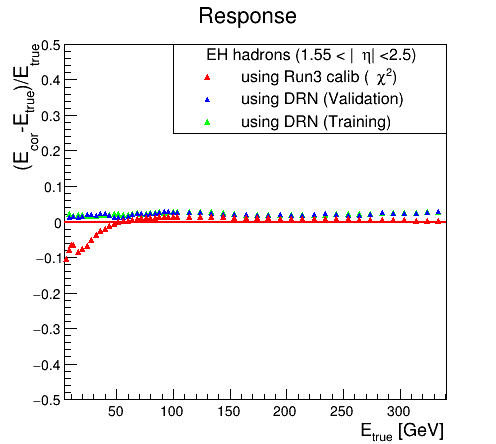
\includegraphics[width=0.495\textwidth]{./plots_pdf/HCAL_plots/Trained_target_ratioflip_0_500_10/pdf/EH_ec_in/EC_within_tracker_corrEtaEndcapEcalHcal.png}
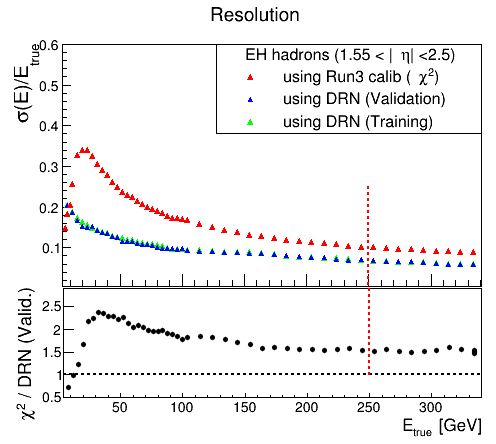
\includegraphics[width=0.495\textwidth]{./plots_pdf/HCAL_plots/Trained_target_ratioflip_0_500_10/pdf/EH_ec_in/EC_within_tracker_corrEtaEndcapEcalHcal_reso.png}
\caption{EH - endcap within tracker - target ratioflip}
\end{figure}


\begin{figure}
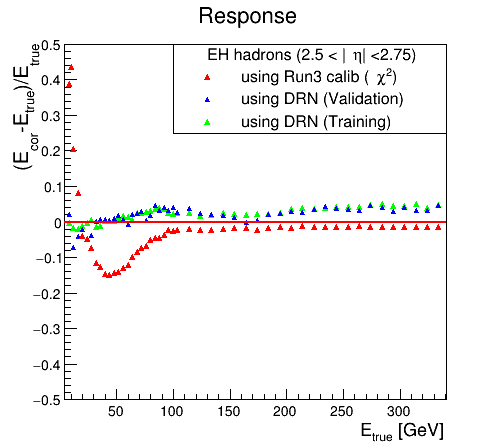
\includegraphics[width=0.495\textwidth]{./plots_pdf/HCAL_plots/Trained_target_ratioflip_0_500_10/pdf/EH_ec_out/EC_outside_tracker_corrEtaEndcapEcalHcal.png}
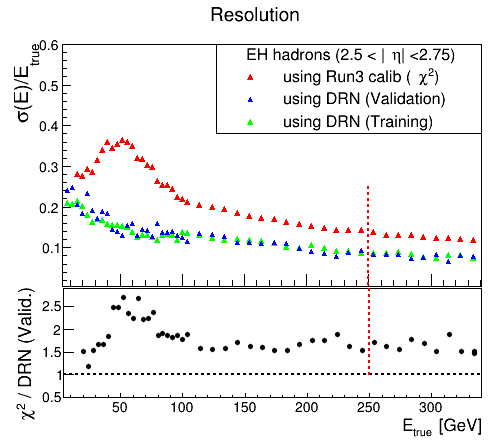
\includegraphics[width=0.495\textwidth]{./plots_pdf/HCAL_plots/Trained_target_ratioflip_0_500_10/pdf/EH_ec_out/EC_outside_tracker_corrEtaEndcapEcalHcal_reso.png}
\caption{EH - endcap outside the tracker - target ratioflip}
\end{figure}

\end{landscape}

\begin{figure}
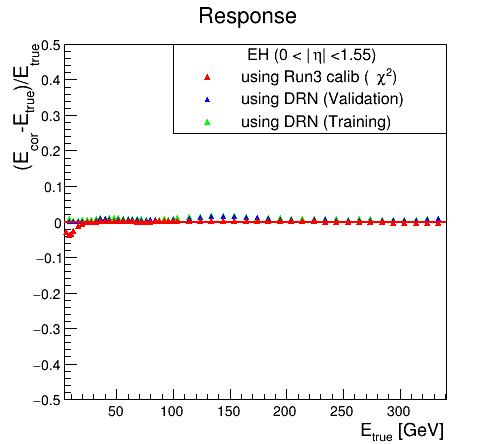
\includegraphics[width=0.495\textwidth]{./plots_pdf/HCAL_plots/Trained_target_ratioflip_0_500_10/pdf/EH_barrel/barrel_corrEtaBarrelEcalHcal.png}
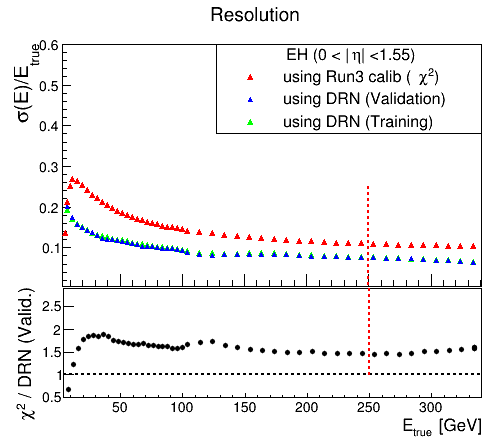
\includegraphics[width=0.495\textwidth]{./plots_pdf/HCAL_plots/Trained_target_ratioflip_0_500_10/pdf/EH_barrel/barrel_corrEtaBarrelEcalHcal_reso.png}
\caption{EH - barrel - target logratioflip}
\end{figure}

\begin{figure}
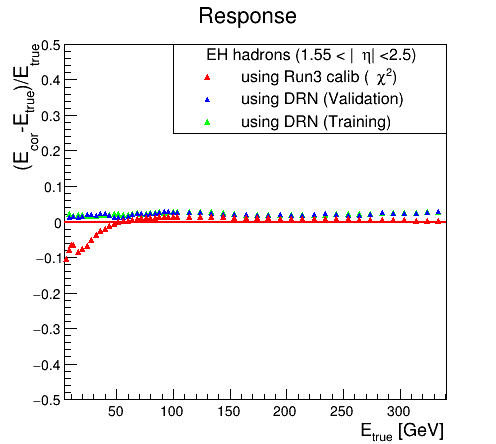
\includegraphics[width=0.495\textwidth]{./plots_pdf/HCAL_plots/Trained_target_ratioflip_0_500_10/pdf/EH_ec_in/EC_within_tracker_corrEtaEndcapEcalHcal.png}
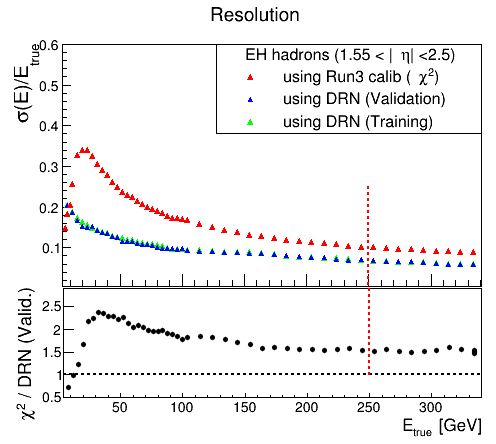
\includegraphics[width=0.495\textwidth]{./plots_pdf/HCAL_plots/Trained_target_ratioflip_0_500_10/pdf/EH_ec_in/EC_within_tracker_corrEtaEndcapEcalHcal_reso.png}
\caption{EH - endcap within tracker - target logratioflip}
\end{figure}


\begin{figure}
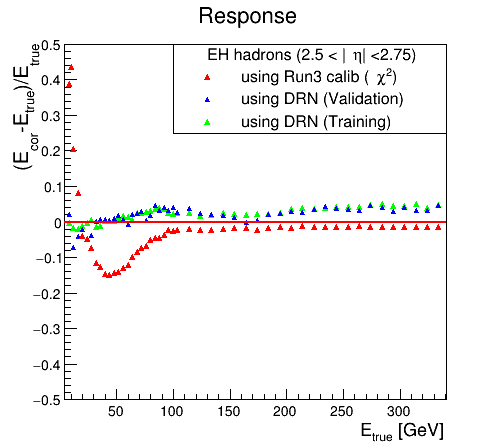
\includegraphics[width=0.495\textwidth]{./plots_pdf/HCAL_plots/Trained_target_ratioflip_0_500_10/pdf/EH_ec_out/EC_outside_tracker_corrEtaEndcapEcalHcal.png}
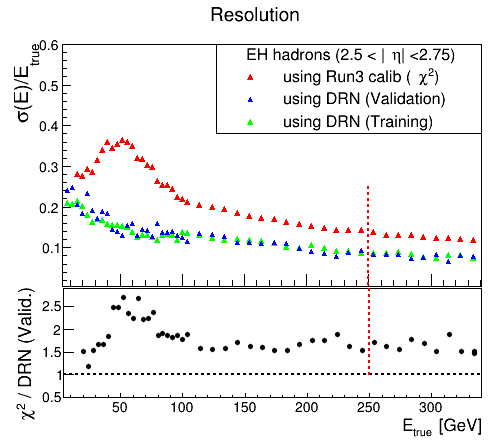
\includegraphics[width=0.495\textwidth]{./plots_pdf/HCAL_plots/Trained_target_ratioflip_0_500_10/pdf/EH_ec_out/EC_outside_tracker_corrEtaEndcapEcalHcal_reso.png}
\caption{EH - endcap outside the tracker - target logratioflip}
\end{figure}

\begin{figure}
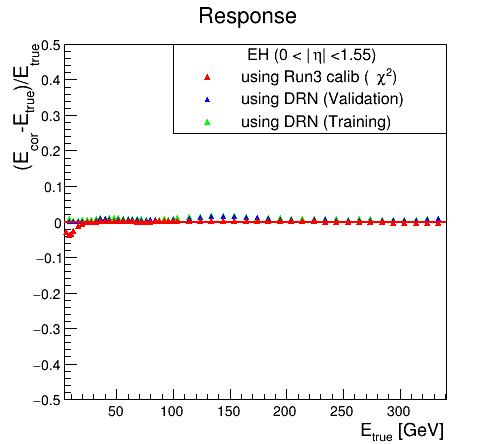
\includegraphics[width=0.495\textwidth]{./plots_pdf/HCAL_plots/Trained_target_ratioflip_0_500_10/pdf/EH_barrel/barrel_corrEtaBarrelEcalHcal.png}
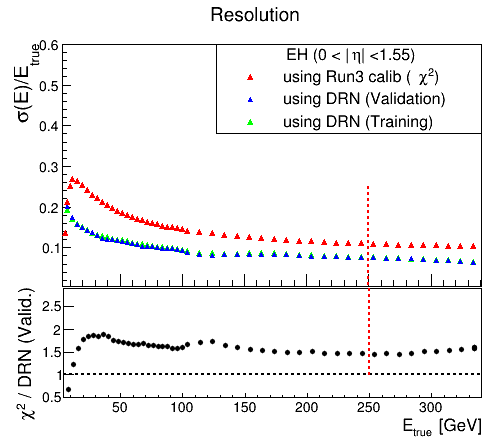
\includegraphics[width=0.495\textwidth]{./plots_pdf/HCAL_plots/Trained_target_ratioflip_0_500_10/pdf/EH_barrel/barrel_corrEtaBarrelEcalHcal_reso.png}
\caption{EH - barrel - target_ratio}                                                                                                                                               
\end{figure}                                                                                                                                                                      

\begin{figure}                                                                                                                                                                   
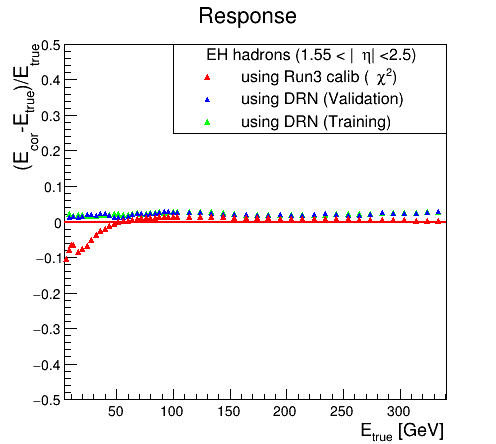
\includegraphics[width=0.495\textwidth]{./plots_pdf/HCAL_plots/Trained_target_ratioflip_0_500_10/pdf/EH_ec_in/EC_within_tracker_corrEtaEndcapEcalHcal.png}
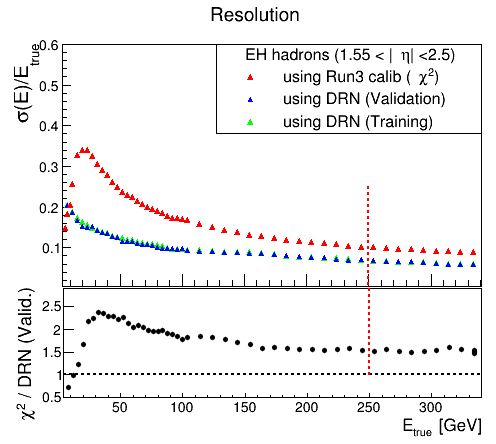
\includegraphics[width=0.495\textwidth]{./plots_pdf/HCAL_plots/Trained_target_ratioflip_0_500_10/pdf/EH_ec_in/EC_within_tracker_corrEtaEndcapEcalHcal_reso.png}
\caption{EH - endcap within tracker - target_ratio}
\end{figure}


\begin{figure}
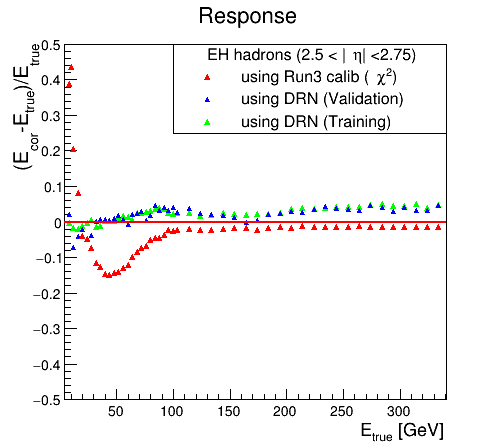
\includegraphics[width=0.495\textwidth]{./plots_pdf/HCAL_plots/Trained_target_ratioflip_0_500_10/pdf/EH_ec_out/EC_outside_tracker_corrEtaEndcapEcalHcal.png}
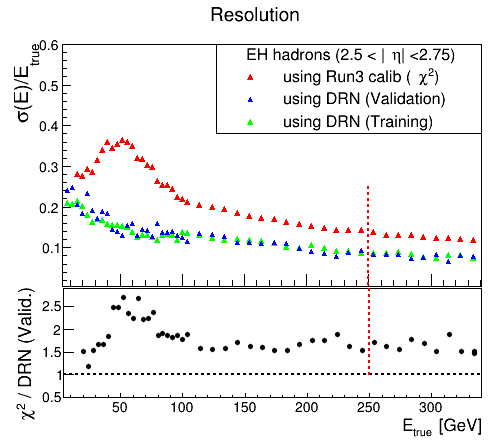
\includegraphics[width=0.495\textwidth]{./plots_pdf/HCAL_plots/Trained_target_ratioflip_0_500_10/pdf/EH_ec_out/EC_outside_tracker_corrEtaEndcapEcalHcal_reso.png}
\caption{EH - endcap outside the tracker - target_ratio}
\end{figure}

\begin{figure}
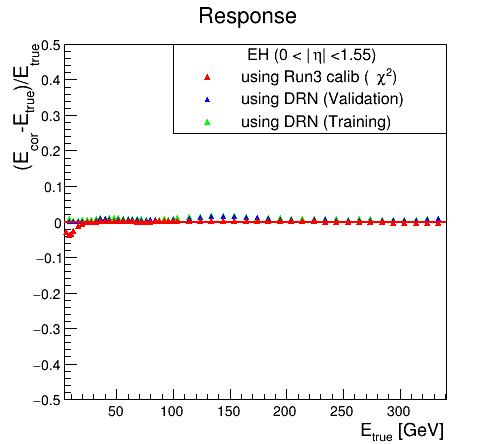
\includegraphics[width=0.495\textwidth]{./plots_pdf/HCAL_plots/Trained_target_ratioflip_0_500_10/pdf/EH_barrel/barrel_corrEtaBarrelEcalHcal.png}
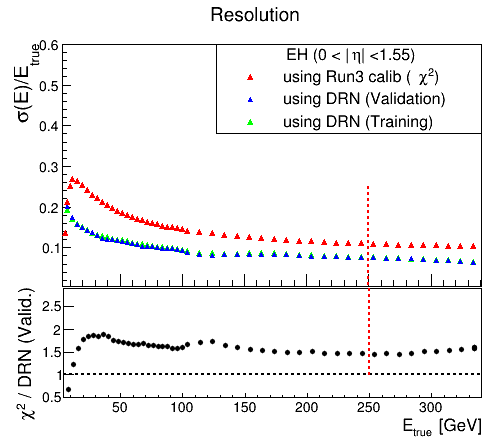
\includegraphics[width=0.495\textwidth]{./plots_pdf/HCAL_plots/Trained_target_ratioflip_0_500_10/pdf/EH_barrel/barrel_corrEtaBarrelEcalHcal_reso.png}
%\caption{EH - barrel - target trueE}
%\end{figure}

%\begin{figure}
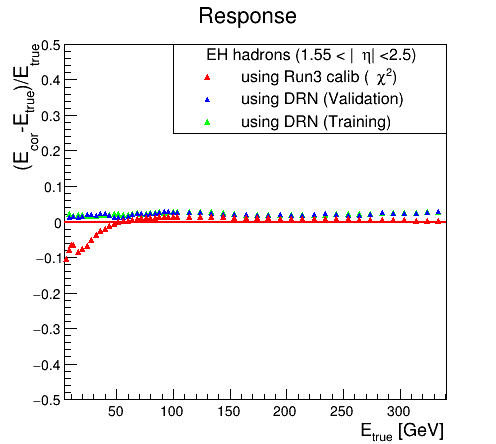
\includegraphics[width=0.495\textwidth]{./plots_pdf/HCAL_plots/Trained_target_ratioflip_0_500_10/pdf/EH_ec_in/EC_within_tracker_corrEtaEndcapEcalHcal.png}
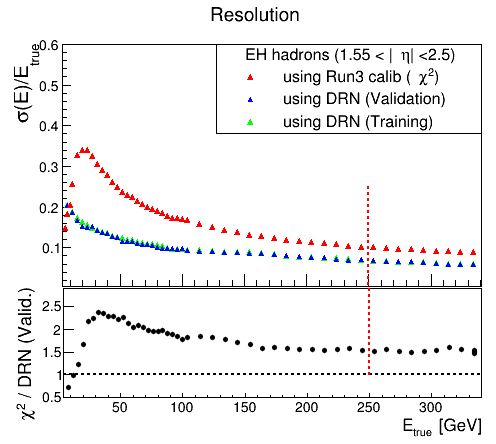
\includegraphics[width=0.495\textwidth]{./plots_pdf/HCAL_plots/Trained_target_ratioflip_0_500_10/pdf/EH_ec_in/EC_within_tracker_corrEtaEndcapEcalHcal_reso.png}
%\caption{EH - endcap within tracker - target trueE}
%\end{figure}


%\begin{figure}
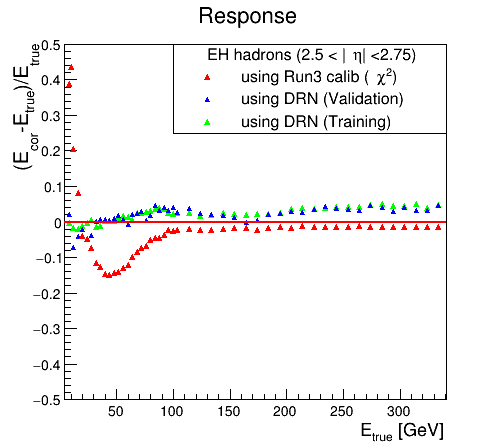
\includegraphics[width=0.495\textwidth]{./plots_pdf/HCAL_plots/Trained_target_ratioflip_0_500_10/pdf/EH_ec_out/EC_outside_tracker_corrEtaEndcapEcalHcal.png}
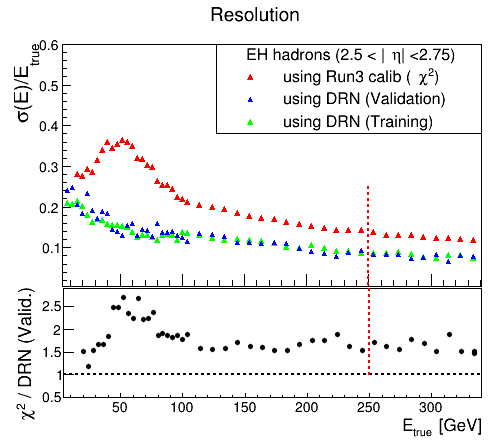
\includegraphics[width=0.495\textwidth]{./plots_pdf/HCAL_plots/Trained_target_ratioflip_0_500_10/pdf/EH_ec_out/EC_outside_tracker_corrEtaEndcapEcalHcal_reso.png}
\caption{EH - (top) barrel, (middle) endcap within tracker, (bottom) endcap outside the tracker - target trueE}
\label{fig:EH_trueE}
\end{figure}


\subsection{H hadrons}
\begin{figure}
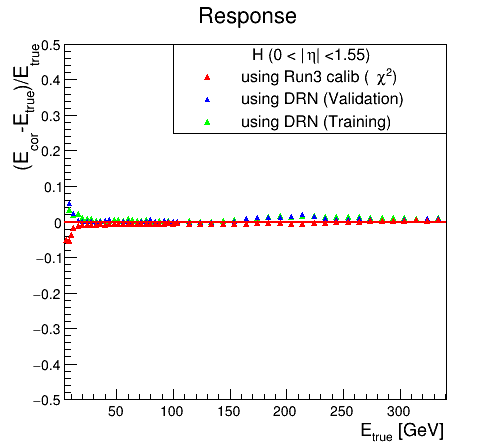
\includegraphics[width=0.495\textwidth]{./plots_pdf/HCAL_plots/Trained_target_ratioflip_0_500_10/pdf/H_barrel/barrel_corrEtaBarrelHcal.png}
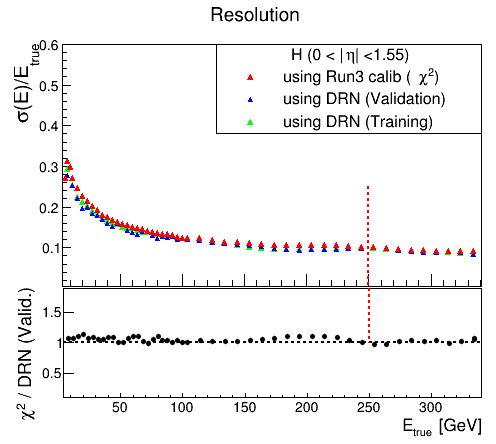
\includegraphics[width=0.495\textwidth]{./plots_pdf/HCAL_plots/Trained_target_ratioflip_0_500_10/pdf/H_barrel/barrel_corrEtaBarrelHcal_reso.png}

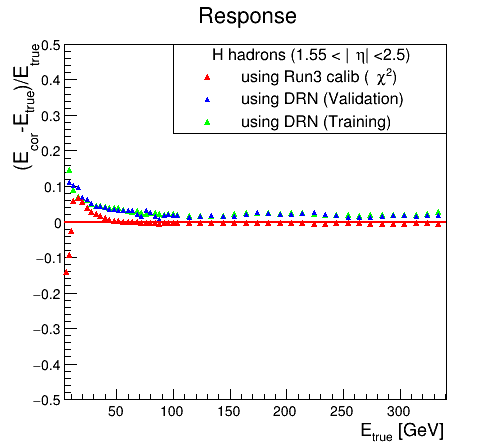
\includegraphics[width=0.495\textwidth]{./plots_pdf/HCAL_plots/Trained_target_ratioflip_0_500_10/pdf/H_ec_in/EC_within_tracker_corrEtaEndcapHcal.png}
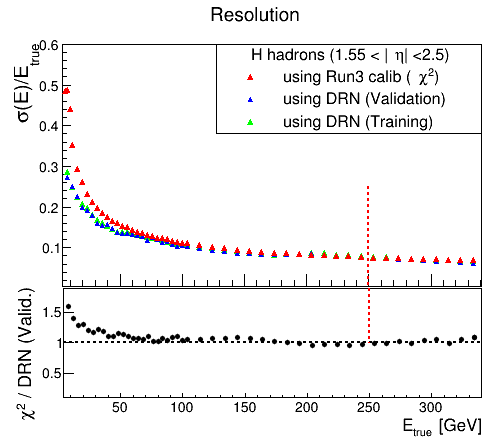
\includegraphics[width=0.495\textwidth]{./plots_pdf/HCAL_plots/Trained_target_ratioflip_0_500_10/pdf/H_ec_in/EC_within_tracker_corrEtaEndcapHcal_reso.png}

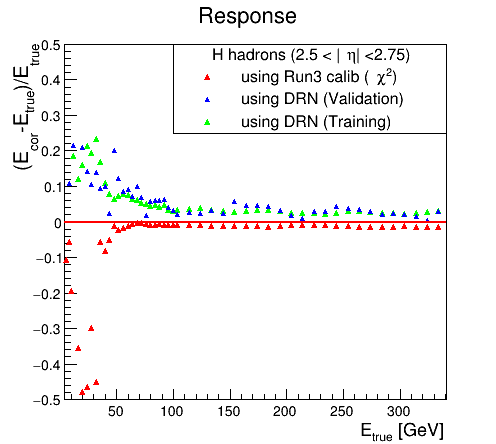
\includegraphics[width=0.495\textwidth]{./plots_pdf/HCAL_plots/Trained_target_ratioflip_0_500_10/pdf/H_ec_out/EC_outside_tracker_corrEtaEndcapHcal.png}
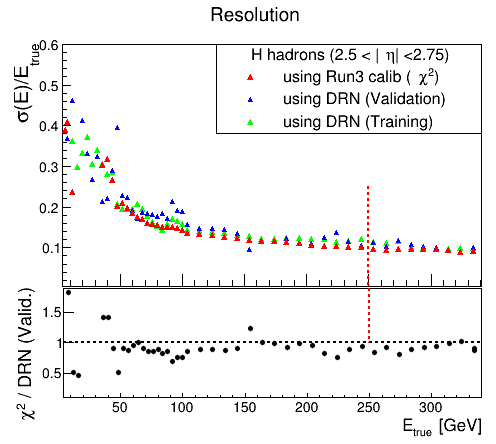
\includegraphics[width=0.495\textwidth]{./plots_pdf/HCAL_plots/Trained_target_ratioflip_0_500_10/pdf/H_ec_out/EC_outside_tracker_corrEtaEndcapHcal_reso.png}

\caption[Energy response (resolution) of the PF H-hadron cluster training traget ratioflip]{H - (top) barrel , (middle) endcap within tracker, (bottom) endcap outside the tracker - target ratioflip}
\label{fig:H_ratioflip}
\end{figure}

\begin{figure}
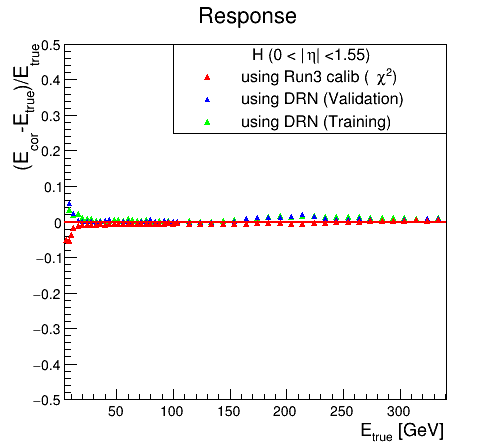
\includegraphics[width=0.495\textwidth]{./plots_pdf/HCAL_plots/Trained_target_ratioflip_0_500_10/pdf/H_barrel/barrel_corrEtaBarrelHcal.png}
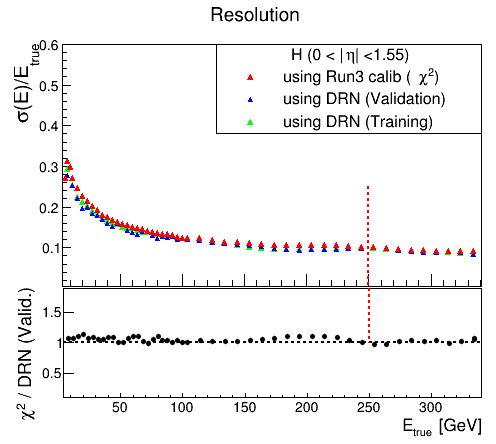
\includegraphics[width=0.495\textwidth]{./plots_pdf/HCAL_plots/Trained_target_ratioflip_0_500_10/pdf/H_barrel/barrel_corrEtaBarrelHcal_reso.png}
\caption{H - barrel - target_logratioflip}                                                                                                                                               
\end{figure}


\begin{figure}                                                                                                                                                               
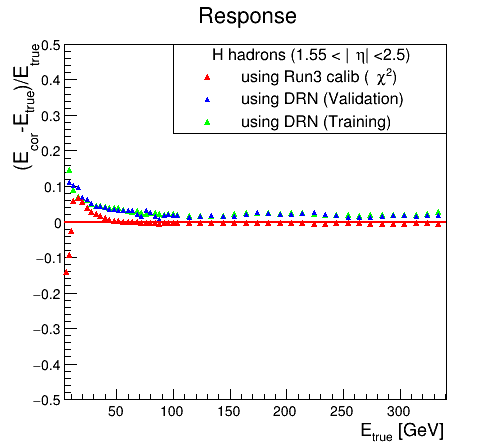
\includegraphics[width=0.495\textwidth]{./plots_pdf/HCAL_plots/Trained_target_ratioflip_0_500_10/pdf/H_ec_in/EC_within_tracker_corrEtaEndcapHcal.png}
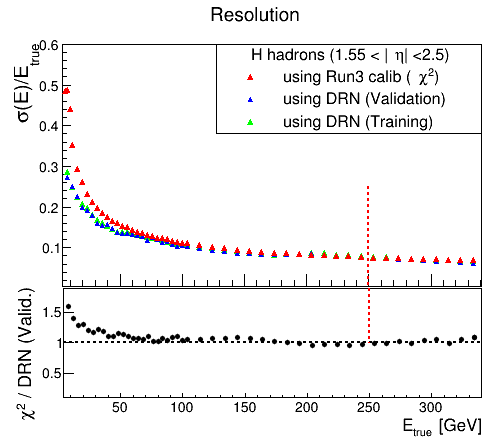
\includegraphics[width=0.495\textwidth]{./plots_pdf/HCAL_plots/Trained_target_ratioflip_0_500_10/pdf/H_ec_in/EC_within_tracker_corrEtaEndcapHcal_reso.png}
\caption{H - endcap within tracker - target_logratioflip}
\end{figure}


\begin{figure}
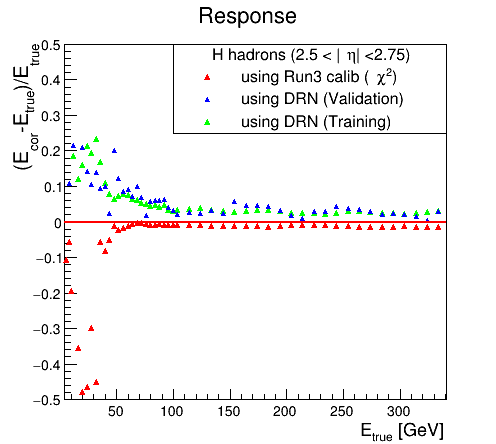
\includegraphics[width=0.495\textwidth]{./plots_pdf/HCAL_plots/Trained_target_ratioflip_0_500_10/pdf/H_ec_out/EC_outside_tracker_corrEtaEndcapHcal.png}
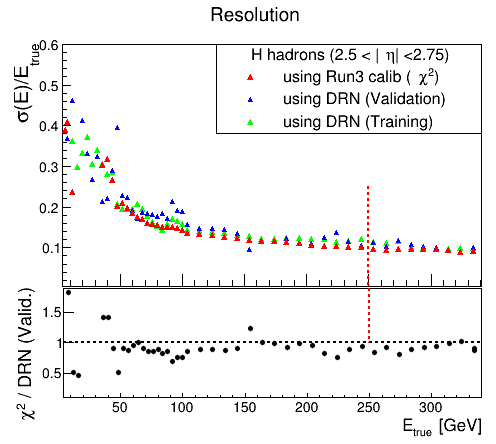
\includegraphics[width=0.495\textwidth]{./plots_pdf/HCAL_plots/Trained_target_ratioflip_0_500_10/pdf/H_ec_out/EC_outside_tracker_corrEtaEndcapHcal_reso.png}
\caption{H - endcap outside the tracker - target_logratioflip}
\end{figure}

\begin{figure}
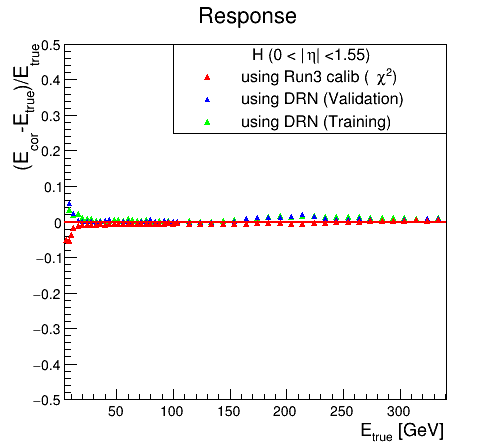
\includegraphics[width=0.495\textwidth]{./plots_pdf/HCAL_plots/Trained_target_ratioflip_0_500_10/pdf/H_barrel/barrel_corrEtaBarrelHcal.png}
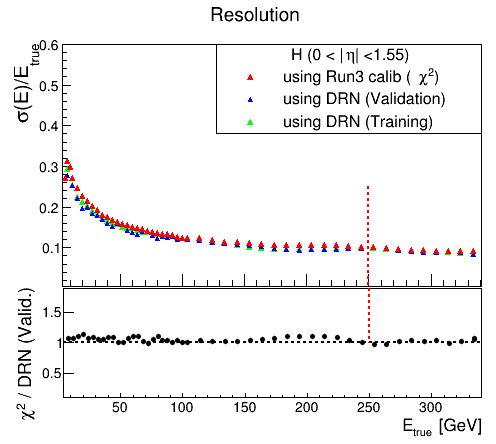
\includegraphics[width=0.495\textwidth]{./plots_pdf/HCAL_plots/Trained_target_ratioflip_0_500_10/pdf/H_barrel/barrel_corrEtaBarrelHcal_reso.png}
%\caption{H - barrel - target ratio}
%\end{figure}


%\begin{figure}
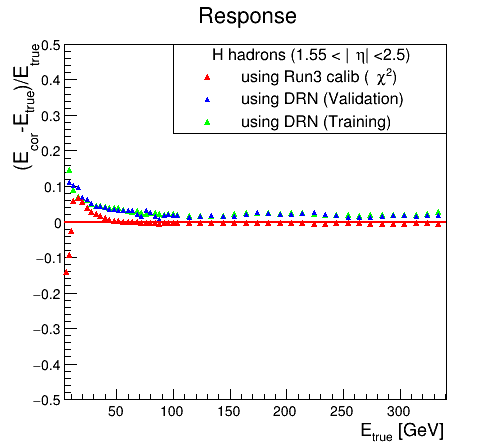
\includegraphics[width=0.495\textwidth]{./plots_pdf/HCAL_plots/Trained_target_ratioflip_0_500_10/pdf/H_ec_in/EC_within_tracker_corrEtaEndcapHcal.png}
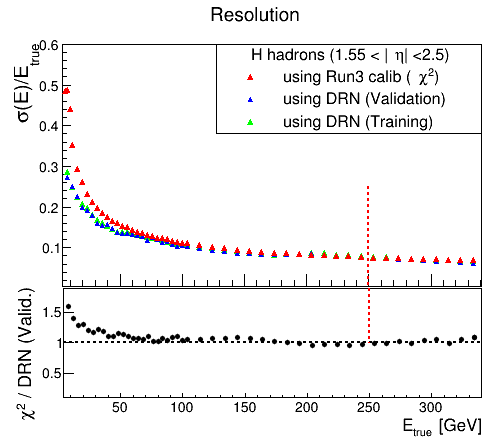
\includegraphics[width=0.495\textwidth]{./plots_pdf/HCAL_plots/Trained_target_ratioflip_0_500_10/pdf/H_ec_in/EC_within_tracker_corrEtaEndcapHcal_reso.png}
%\caption{H - endcap within tracker - target ratio}
%\end{figure}


%\begin{figure}
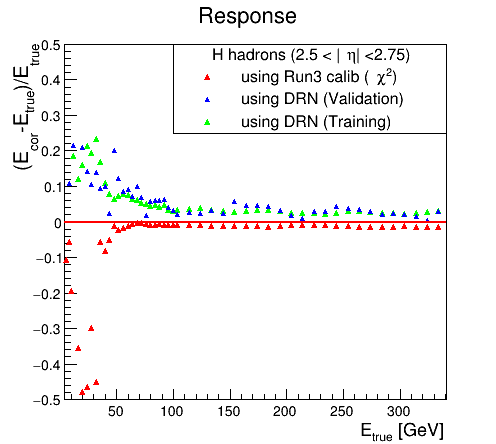
\includegraphics[width=0.495\textwidth]{./plots_pdf/HCAL_plots/Trained_target_ratioflip_0_500_10/pdf/H_ec_out/EC_outside_tracker_corrEtaEndcapHcal.png}
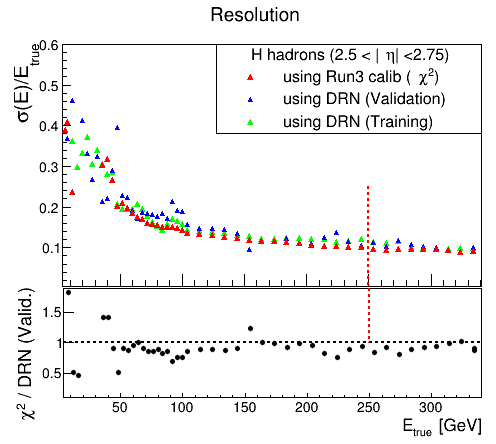
\includegraphics[width=0.495\textwidth]{./plots_pdf/HCAL_plots/Trained_target_ratioflip_0_500_10/pdf/H_ec_out/EC_outside_tracker_corrEtaEndcapHcal_reso.png}
\caption{H - (top) barrel, (middle) endcap within tracker, (bottom) endcap outside the tracker - target ratio}
\end{figure}

\begin{figure}
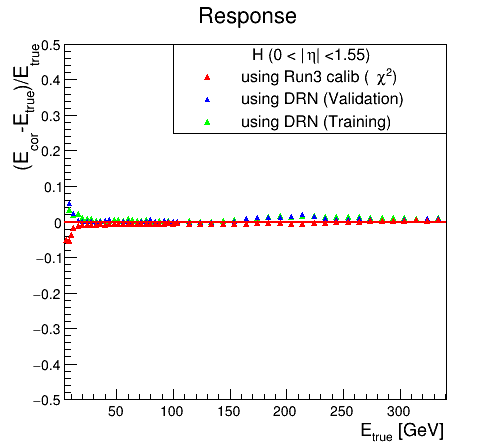
\includegraphics[width=0.495\textwidth]{./plots_pdf/HCAL_plots/Trained_target_ratioflip_0_500_10/pdf/H_barrel/barrel_corrEtaBarrelHcal.png}
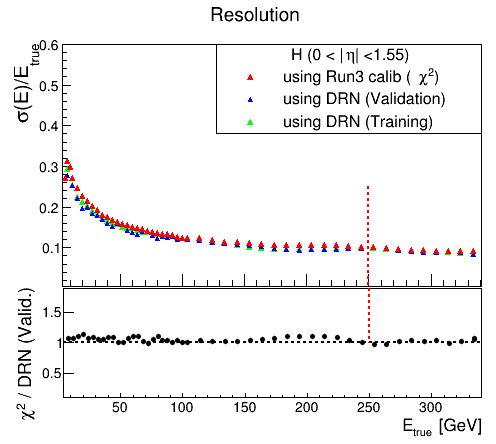
\includegraphics[width=0.495\textwidth]{./plots_pdf/HCAL_plots/Trained_target_ratioflip_0_500_10/pdf/H_barrel/barrel_corrEtaBarrelHcal_reso.png}
\caption{H - barrel - target_trueE}                                                                                                                                               
\end{figure}


\begin{figure}                                                                                                                                                               
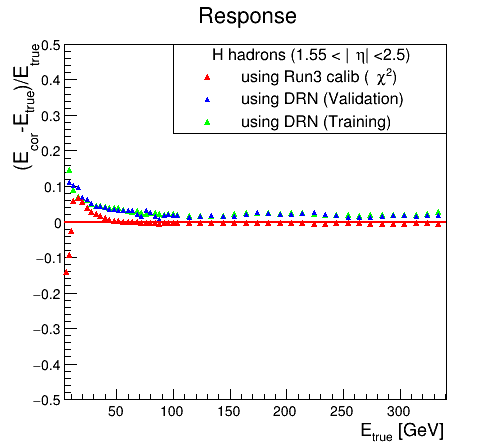
\includegraphics[width=0.495\textwidth]{./plots_pdf/HCAL_plots/Trained_target_ratioflip_0_500_10/pdf/H_ec_in/EC_within_tracker_corrEtaEndcapHcal.png}
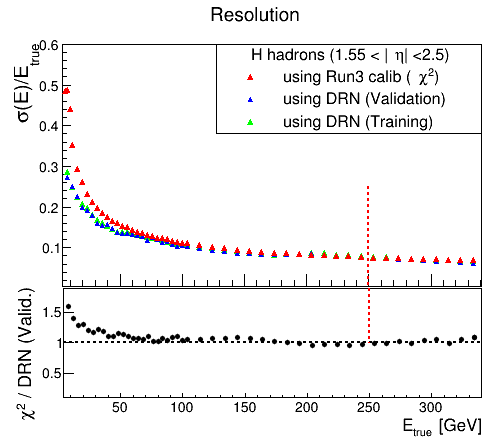
\includegraphics[width=0.495\textwidth]{./plots_pdf/HCAL_plots/Trained_target_ratioflip_0_500_10/pdf/H_ec_in/EC_within_tracker_corrEtaEndcapHcal_reso.png}
\caption{H - endcap within tracker - target_trueE}
\end{figure}


\begin{figure}
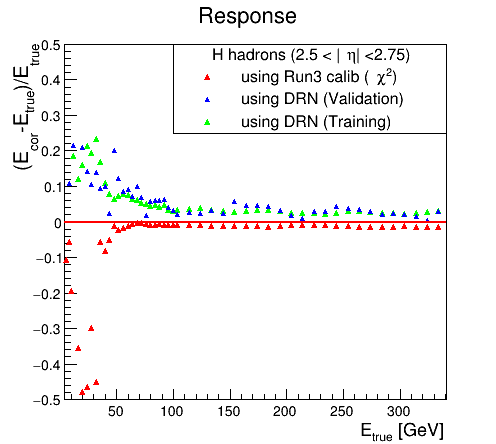
\includegraphics[width=0.495\textwidth]{./plots_pdf/HCAL_plots/Trained_target_ratioflip_0_500_10/pdf/H_ec_out/EC_outside_tracker_corrEtaEndcapHcal.png}
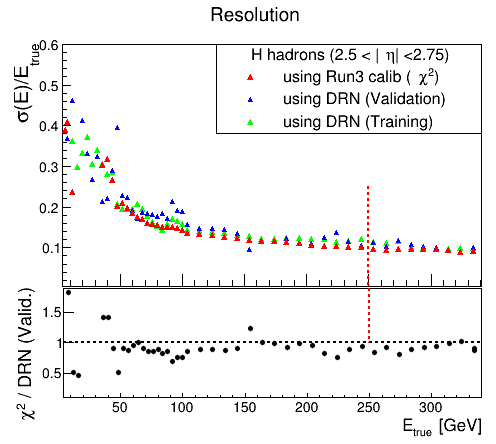
\includegraphics[width=0.495\textwidth]{./plots_pdf/HCAL_plots/Trained_target_ratioflip_0_500_10/pdf/H_ec_out/EC_outside_tracker_corrEtaEndcapHcal_reso.png}
\caption{H - endcap outside the tracker - target_trueE}
\end{figure}

